%!TEX root = ../../main.tex
\begin{figure}[h]
    \centering
    \begin{subfigure}[b]{1\textwidth}
    \centering
    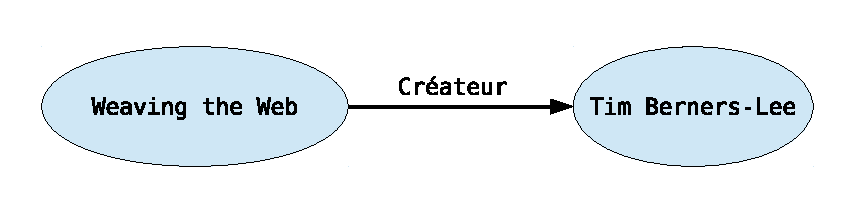
\includegraphics[width=0.85\textwidth]{figs/A/rdf-statement-example-graph.eps}
    \caption{Illustaion graphique d'une assertion \acrshort{rdf}.}
    \label{fig:rdf-statement-example-graph}
    \end{subfigure}

    \begin{subfigure}[b]{1\textwidth}
      \centering
      \lstinputlisting[language={XML}]{figs/A/rdf-statement-example.rdf}
      \caption{Document RDF/XMl \acrshort{rdf}.}
      \label{fig:rdf-statement-example-graph}
    \end{subfigure}

    \caption{Un exeample d'une assertion \acrshort{rdf}}
    \label{fig:rdf-statement-example}
\end{figure}
%%% Local Variables:
%%% mode: latex
%%% TeX-master: "../../main"
%%% End:
